\documentclass{article}
\usepackage{amsmath}

\usepackage{graphicx}

\usepackage{listings}
\usepackage{color}
\definecolor{dkgreen}{rgb}{0,0.6,0}
\definecolor{gray}{rgb}{0.5,0.5,0.5}
\definecolor{mauve}{rgb}{0.58,0,0.82}
\lstset{frame=tb,
  language=R,
  aboveskip=3mm,
  belowskip=3mm,
  showstringspaces=false,
  columns=flexible,
  basicstyle={\small\ttfamily},
  numbers=none,
  numberstyle=\tiny\color{gray},
  keywordstyle=\color{blue},
  commentstyle=\color{dkgreen},
  stringstyle=\color{mauve},
  breaklines=false,
  breakatwhitespace=true,
  tabsize=3
}

\title{SDS385 Fall '16: Statistical Models For Big Data\\Exercises 02 - SGD for logistic regression}
\author{Matteo Vestrucci}
\date{September 14th 2016}
\begin{document}
\maketitle
\bigskip\bigskip\bigskip

\subsubsection*{A)}

Using the same proof of the last time, the gradient can be written as

\begin{align*}
\nabla l(\beta)&=\nabla\left(\sum_{i=1}^N (m_i-y_i) x_i^T\beta+\sum_{i=1}^N m_i \log(1+e^{-x_i^T\beta})\right)\\
				&=\sum_{i=1}^N (m_i-y_i) x_i+\sum_{i=1}^N m_i w_i e^{-x_i^T\beta}(-x_i)\\
				&=\sum_{i=1}^N m_i x_i-\sum_{i=1}^N y_i x_i-\sum_{i=1}^N m_i (1-w_i) x_i\\
				&=-\sum_{i=1}^N y_i x_i+\sum_{i=1}^N m_i w_i x_i\\
				&=\sum_{i=1}^N (m_i w_i-y_i)x_i=\sum_{i=1}^N (\hat{y}-y_i)x_i\\
\end{align*}

\subsubsection*{B)}

Using the second framework where the pairs $(y_i,x_i)$ are $i.i.d$ samples from the same distribution, the proof for the statement is the following:

\begin{equation*}
\text{E}[ng_i(\beta)]=n\text{E}[(\hat{y_i}-y_i)x_i]=n\frac{\sum_i (\hat{y_i}-y_i)x_i}{n}={\sum}_i g_i(\beta)=\nabla l(\beta)
\end{equation*}

\subsubsection*{C)}

Running the code in appendix, $100000$ iterations without any other stopping condition, we can observe how the stochastic gradient descent with fixed step behaves.

\begin{center}
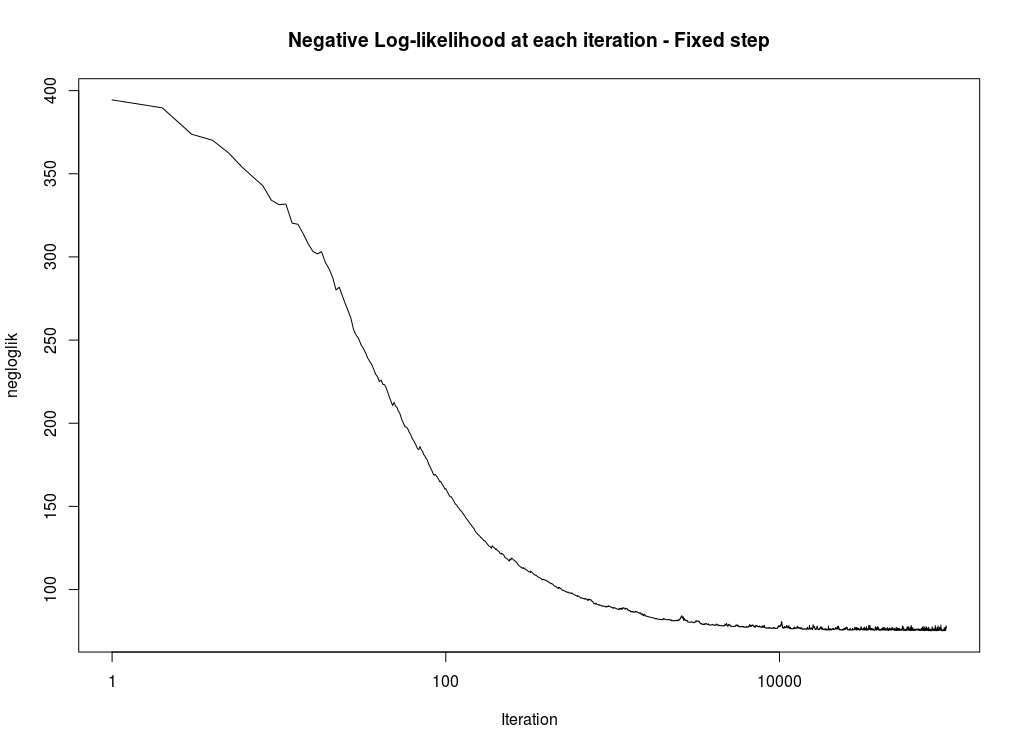
\includegraphics[width=0.8\textwidth]{Rplot_total_negloglik.png} 
\end{center}

This first picture clearly shows a not strictly descending path, especially after reaching pseudo-convergence. A possible interpretation is that the proposed optimum keeps jumping freely around the real optimum depending on which unit is selected at that specific time. The second picture instead shows the running average of the negative loglikelihood for the single randomly selected unit, rescaled multiplying by $n$ to be comparable with the previous plot. 

\begin{center}
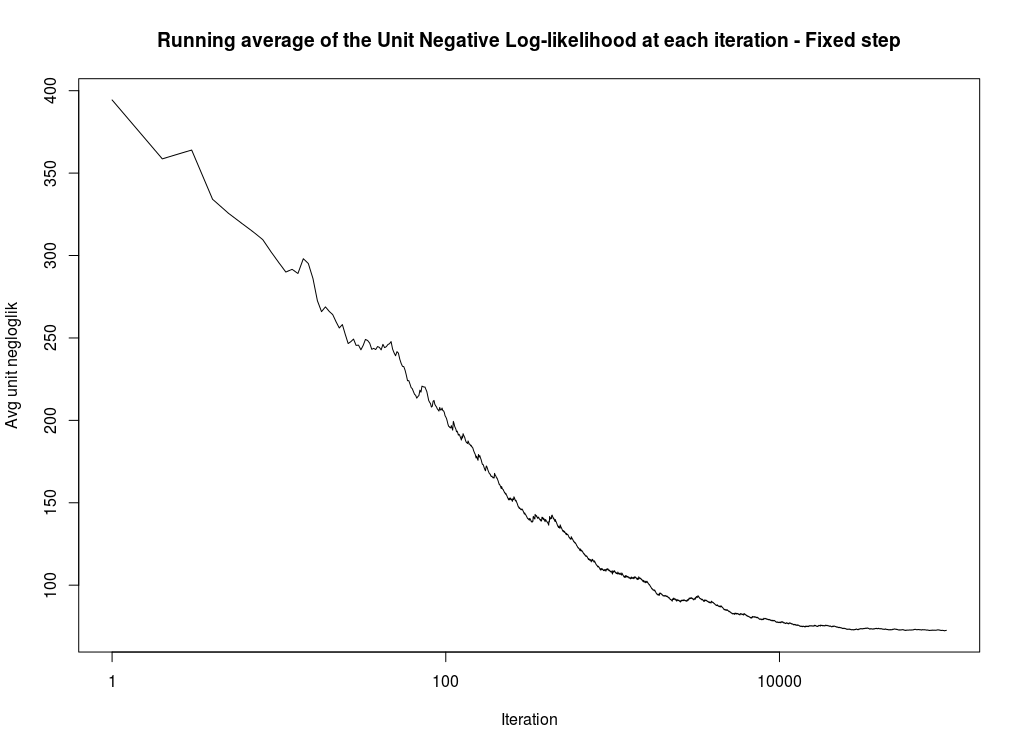
\includegraphics[width=0.8\textwidth]{Rplot_run_avg_unit_negloglik.png}
\end{center}


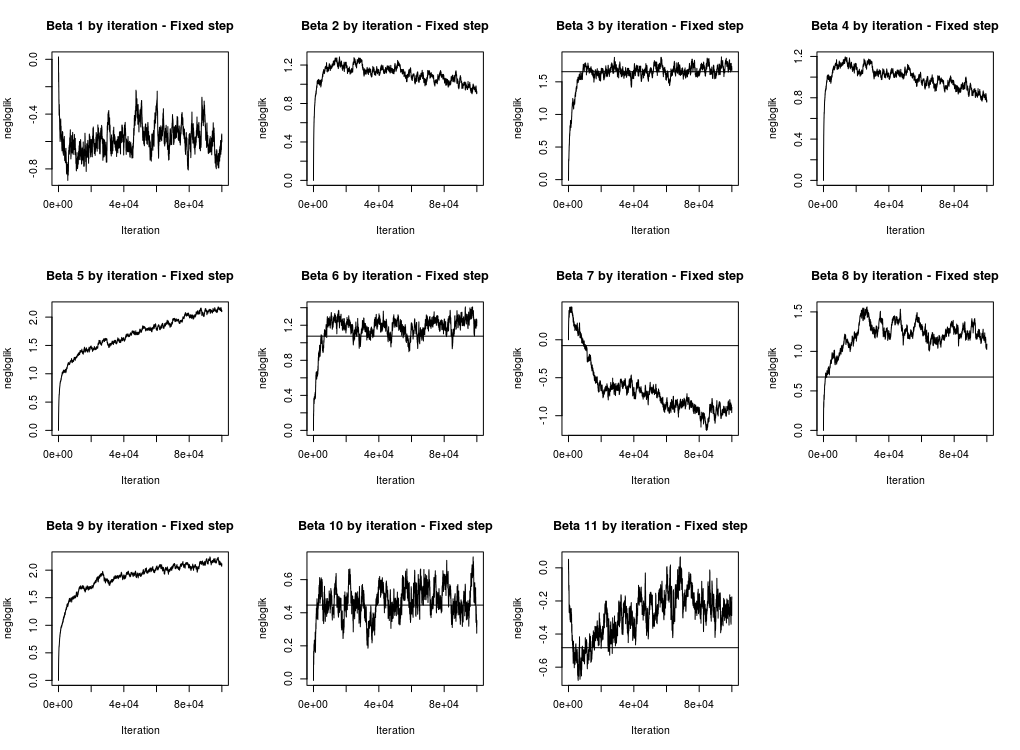
\includegraphics[width=\textwidth]{Rplot_beta_traces.png}

This picture shows how the betas change at each step. Every beta seems to approach a certain degree of stability, but the values are often far away from the GLM estimates (they are represented by horizontal lines only if within the plot range). One explanation of what is happening may be that the objective function is very flat at the bottom which makes the negative loglikelihood to be almost the same for very different combinations of beta values.

\subsubsection*{D)}

The implementation of the Robbins-Monroe rule for the decaying step size requires $C$ and $a$: the first represents how big is going to be what we could call the reference step. At every iteration its size is shrunk at a speed dictated by $a$. As a comparison, in the previous implementation we used a fixed step of size $0.02$ and these are the values obtained setting $C=5$ and $a=0.8$.

\begin{center}
\begin{tabular}{ll}
Iteration  &Step size\\
1          &2.871746\\
10         &0.7342701\\
100        &0.1245985\\
500        &0.03460189\\
1000       &0.01988945\\
5000       &0.005491924\\
10000      &0.003154534\\
50000      &0.0008705366\\
100000     &0.000499996
\end{tabular}
\end{center}

Running the code in appendix, again $100000$ iterations without any other stopping condition, we observed the following results about the stochastic gradient descent with decaying step:

\begin{center}
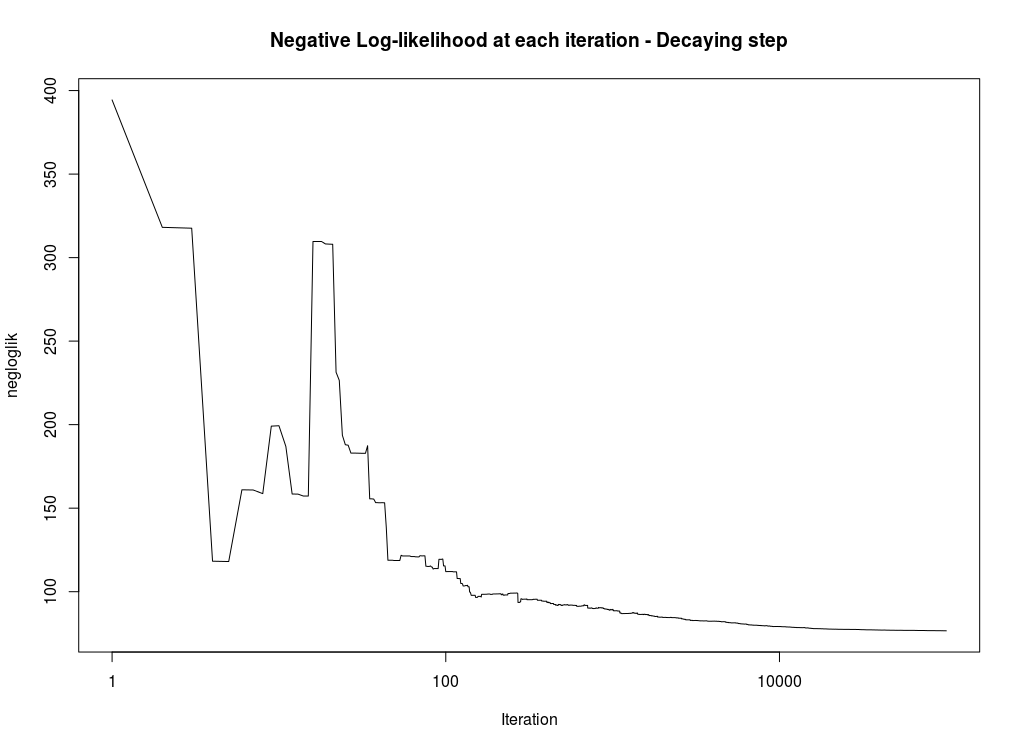
\includegraphics[width=0.8\textwidth]{Rplot_total_negloglik2.png} 
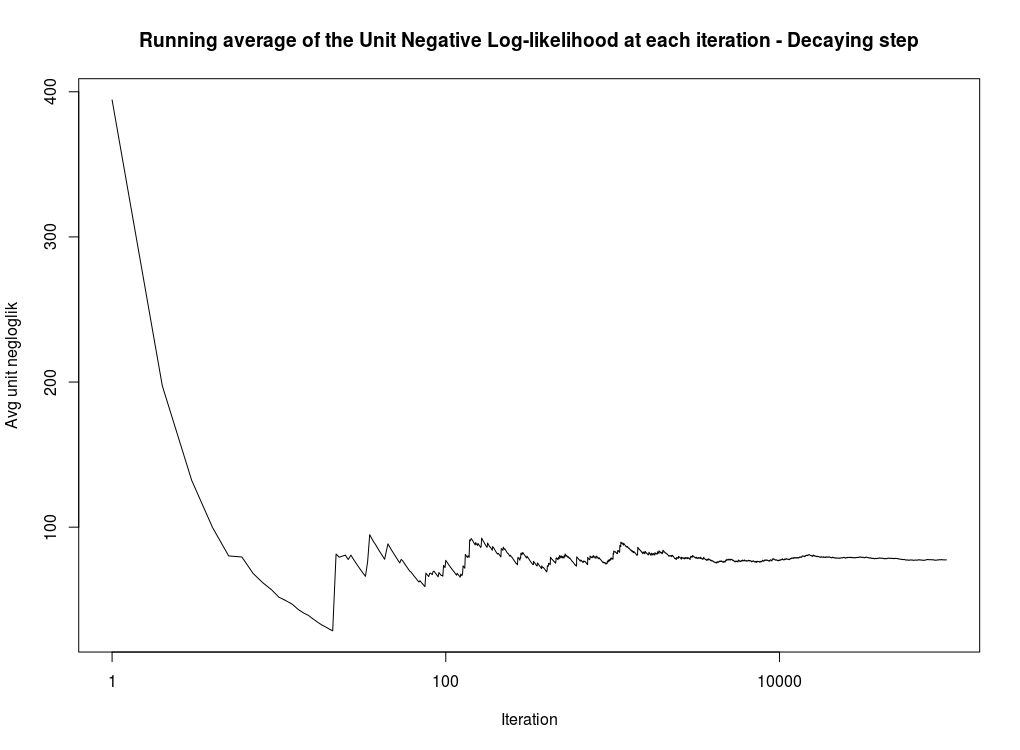
\includegraphics[width=0.8\textwidth]{Rplot_run_avg_unit_negloglik2.png}
\end{center}

As before, the first picture represents the complete negative loglikelihood while the second picture instead shows the running average of the negative loglikelihood for the single randomly selected unit, rescaled multiplying by $n$ to be comparable with the previous plot. Even more clearly than before, it's not a strictly descending path. Being forced to use $t_0=1$ makes the first 100 steps quite big, and that in addiction to using a single unit to find the gradient makes our candidate optimums move all over the sample space. Still convergence is reached well before the max number of iterations. 

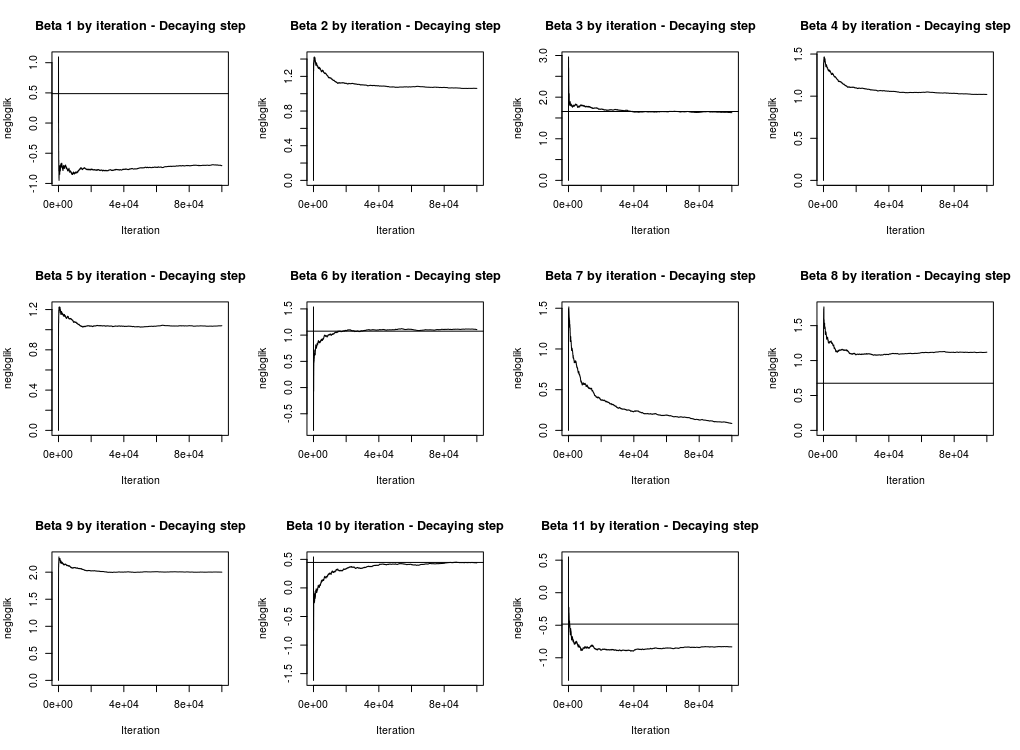
\includegraphics[width=\textwidth]{Rplot_beta_traces2.png}

The fact that the step is decaying, makes the beta traces much more stable because the movements at each iteration become smaller and smaller. Again the values are often different from the GLM estimates, the horizontal lines.

\subsubsection*{E)}

Running the last portion of the code, the Polyak-Ruppert averaging, on the same $\beta$s obtained from the SGD with fixed step and decaying step, we can obtain the following graphs:

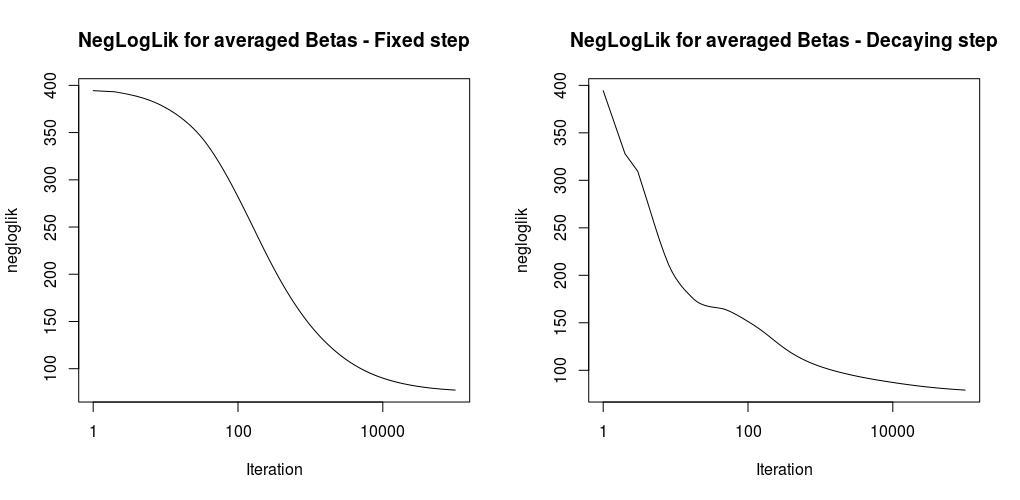
\includegraphics[width=\textwidth]{Rplot_negloglik_avg_beta.png}

Averaging the $\beta$s makes the convergence slower but definitely more stable.

\newpage

\subsubsection*{CODE)}

\begin{lstlisting}[basicstyle=\tiny]
negloglikelihood<-function(m,y,X,beta){
  total<-0
  N<-length(y)
  for(i in 1:N)
  	total<-total+(m[i]-y[i])*t(X[i,])%*%beta+m[i]*log(1+exp(-t(X[i,])%*%beta))
  return(total)
}

unit_negloglikelihood<-function(m,y,X,beta,unit){
  result<-(m[unit]-y[unit])*t(X[unit,])%*%beta+m[unit]*log(1+exp(-t(X[unit,])%*%beta))
  return(result)
}

unit_gradient_negloglik<-function(m,y,X,beta,unit){
  unitX<-X[unit,]
  unitY<-y[unit]
  unitM<-m[unit]
  unitW<-1/(1+exp(-crossprod(unitX,beta)))
  S<-unitM*unitW-unitY
  grad<-unitX*S
  return(grad)
}

stocastic_gradient_descent<-function(m,y,X,beta0,stepsize,maxstepnumber){
  n<-dim(X)[1]
  unit<-sample(seq(1,n),1)
  betas<-matrix(NA,nrow=maxstepnumber,ncol=dim(X)[2])
  betas[1,]<-beta0
  negloglik<-numeric(maxstepnumber)
  negloglik[1]<-negloglikelihood(m,y,X,beta0)
  unit_negloglik<-numeric(maxstepnumber)
  unit_negloglik[1]<-negloglik[1]/n
  gradient<-unit_gradient_negloglik(m,y,X,beta0,unit)
  i<-1
  while(!(i==maxstepnumber)){
    i<-i+1
    beta1<-beta0-stepsize*gradient
    beta0<-beta1
    negloglik[i]<-negloglikelihood(m,y,X,beta0)
    unit_negloglik[i]<-unit_negloglikelihood(m,y,X,beta0,unit)
    betas[i,]<-beta0
    unit<-sample(seq(1,n),1)
    gradient<-unit_gradient_negloglik(m,y,X,beta0,unit)
  }
  return(list(betahat=beta0,negloglik=negloglik,
              unit_negloglik=unit_negloglik,betas=betas,step=i))
}

data_wdbc<-read.csv("./wdbc.csv", header=FALSE)
X<-as.matrix(cbind(rep(1,569),scale(data_wdbc[,3:12])))
y<-data_wdbc[,2]
y<-as.numeric(y=="M")
m<-rep(1,569)

beta0<-rep(0,11)
stepsize<-0.02
maxstepnumber<-100000
res_stoc_grad_desc<-stocastic_gradient_descent(m,y,X,beta0,stepsize,maxstepnumber)

plot(res_stoc_grad_desc$negloglik[1:res_stoc_grad_desc$step],
     main = "Negative Log-likelihood at each iteration - Fixed step",
     xlab="Iteration",ylab="negloglik",type="l",log="x")

running_avg_fix<-numeric(maxstepnumber)
running_avg_fix[1]<-res_stoc_grad_desc$unit_negloglik[1]
for(i in 2:maxstepnumber){
  running_avg_fix[i]<-(running_avg_fix[i-1]*(i-1)+res_stoc_grad_desc$unit_negloglik[i])/(i)}
plot(569*running_avg_fix[1:res_stoc_grad_desc$step],
     main = "Running average of the Unit Negative Log-likelihood at each iteration - Fixed step",
     xlab="Iteration",ylab="Avg unit negloglik",type="l",log="x")

par(mfrow=c(3,4))
estimates<-glm(y~0+X,family='binomial')$coefficients
for(i in 1:11){
plot(res_stoc_grad_desc$betas[1:res_stoc_grad_desc$step,i],
     main = paste("Beta",i,"by iteration - Fixed step"),
     xlab="Iteration",ylab="negloglik",type="l")
abline(h=estimates[i])}
par(mfrow=c(1,1))

robbins_monro_step<-function(iter,C,a){
  weight<-C*(iter+1)^-a
  return(weight)
}



sgd_decaying_step<-function(m,y,X,beta0,C,a,maxstepnumber){
  n<-dim(X)[1]
  unit<-sample(seq(1,n),1)
  betas<-matrix(NA,nrow=maxstepnumber,ncol=dim(X)[2])
  betas[1,]<-beta0
  negloglik<-numeric(maxstepnumber)
  negloglik[1]<-negloglikelihood(m,y,X,beta0)
  unit_negloglik<-numeric(maxstepnumber)
  unit_negloglik[1]<-negloglik[1]/n
  gradient<-unit_gradient_negloglik(m,y,X,beta0,unit)
  i<-1
  while(!(i==maxstepnumber)){
    i<-i+1
    beta1<-beta0-robbins_monro_step(i,C,a)*gradient
    beta0<-beta1
    negloglik[i]<-negloglikelihood(m,y,X,beta0)
    unit_negloglik[i]<-unit_negloglikelihood(m,y,X,beta0,unit)
    betas[i,]<-beta0
    unit<-sample(seq(1,n),1)
    gradient<-unit_gradient_negloglik(m,y,X,beta0,unit)
  }
  return(list(betahat=beta0,negloglik=negloglik,
              unit_negloglik=unit_negloglik,betas=betas,step=i))
}

C<-5
a<-0.8
beta0<-rep(0,11)
maxstepnumber<-100000
res_sgd_decaying_step<-sgd_decaying_step(m,y,X,beta0,C,a,maxstepnumber)

plot(res_sgd_decaying_step$negloglik[1:res_sgd_decaying_step$step],
     main = "Negative Log-likelihood at each iteration - Decaying step",
     xlab="Iteration",ylab="negloglik",type="l",log="x")

running_avg_decay<-numeric(maxstepnumber)
running_avg_decay[1]<-res_sgd_decaying_step$unit_negloglik[1]
for(i in 2:maxstepnumber){
  running_avg_decay[i]<-(running_avg_decay[i-1]*(i-1)+res_sgd_decaying_step$unit_negloglik[i])/(i)}
plot(569*running_avg_decay[1:res_sgd_decaying_step$step],
     main = "Running average of the Unit Negative Log-likelihood at each iteration - Decaying step",
     xlab="Iteration",ylab="Avg unit negloglik",type="l",log="x")

par(mfrow=c(3,4))
estimates<-glm(y~0+X,family='binomial')$coefficients
for(i in 1:11){
  plot(res_sgd_decaying_step$betas[1:res_sgd_decaying_step$step,i],
       main = paste("Beta",i,"by iteration - Decaying step"),
       xlab="Iteration",ylab="negloglik",type="l")
  abline(h=estimates[i])}
par(mfrow=c(1,1))

running_avg_beta_fix<-matrix(NA,nrow=maxstepnumber,ncol=11)
running_avg_beta_decay<-matrix(NA,nrow=maxstepnumber,ncol=11)
running_avg_beta_fix[1,]<-res_stoc_grad_desc$betas[1,]
running_avg_beta_decay[1,]<-res_sgd_decaying_step$betas[1,]
estimates<-glm(y~0+X,family='binomial')$coefficients
for(i in 2:maxstepnumber){
  running_avg_beta_fix[i,]<-(running_avg_beta_fix[i-1,]*(i-1)+res_stoc_grad_desc$betas[i,])/(i)
  running_avg_beta_decay[i,]<-(running_avg_beta_decay[i-1,]*(i-1)+res_sgd_decaying_step$betas[i,])/(i)}
running_negloglik_fix<-numeric(maxstepnumber)
running_negloglik_decay<-numeric(maxstepnumber)
running_negloglik_fix[1]<-negloglikelihood(m,y,X,running_avg_beta_fix[1,])
running_negloglik_decay[1]<-negloglikelihood(m,y,X,running_avg_beta_decay[1,])
for(i in 2:maxstepnumber){
  running_negloglik_fix[i]<-(running_negloglik_fix[i-1]*(i-1)+negloglikelihood(m,y,X,running_avg_beta_fix[i,]))/(i)
  running_negloglik_decay[i]<-(running_negloglik_decay[i-1]*(i-1)+negloglikelihood(m,y,X,running_avg_beta_decay[i,]))/(i)}
par(mfrow=c(1,2))
plot(running_negloglik_fix[1:res_stoc_grad_desc$step],
     main = "NegLogLik for averaged Betas - Fixed step",
     xlab="Iteration",ylab="negloglik",type="l",log="x")
plot(running_negloglik_decay[1:res_sgd_decaying_step$step],
     main = "NegLogLik for averaged Betas - Decaying step",
     xlab="Iteration",ylab="negloglik",type="l",log="x")
par(mfrow=c(1,1))
\end{lstlisting}

\end{document}